\documentclass[a4j,11pt]{ltjsarticle}
\usepackage{luatexja} % ltjclasses, ltjsclasses を使うときはこの行不要

% 正しいA4サイズを余白設定付きで使う設定
% ドライバを指定,余白の設定
\usepackage[top=10truemm,
						bottom=18truemm,
						left=20truemm,
						right=20truemm]{geometry}
\usepackage{graphicx}		% 画像用

\usepackage[T1]{fontenc}		% [記号文字化けを防ぐ]
\usepackage{lmodern}		% [記号文字化けを防ぐ](Latin Modern フォントを使う)
\usepackage{enumerate}	% 数式
\usepackage{comment}		% 複数行コメントアウト
%\usepackage{ascmac} 		% 枠囲み(例:itembox)
%\usepackage{listings}		% [ソースコード挿入] jlistings.styが必要
%\usepackage{listings,jlisting} % [ソースコード挿入] jlistings.styが必要
%\usepackage{amsmath} 		% 行列式の記述用
\begin{comment}
% ソースコードのスタイルの設定
\lstset{%
    language={},
    basicstyle={\small},%
    identifierstyle={\small},%
    commentstyle={\small\itshape},%
    keywordstyle={\small\bfseries},%
    ndkeywordstyle={\small},%
    stringstyle={\small\ttfamily},
    frame={tb},
    breaklines=true,
    columns=[l]{fullflexible},%
    numbers=left,%
    xrightmargin=0zw,%
    xleftmargin=3zw,%
    numberstyle={\scriptsize},%
    stepnumber=1,
    numbersep=1zw,%
    lineskip=-0.5ex%
}
\end{comment}

\begin{document}
    \section{はじめてのLua\TeX-ja}
        ちゃんと日本語が出るかな?

        \subsection{出たかな?}
            長い文章を入力するとちゃんと右端のところで折り返されるかな?
            大丈夫そうな気がするけど.ちょっと不安だけど何事も挑戦だよね.

            \begin{figure}[h]
                \centering
                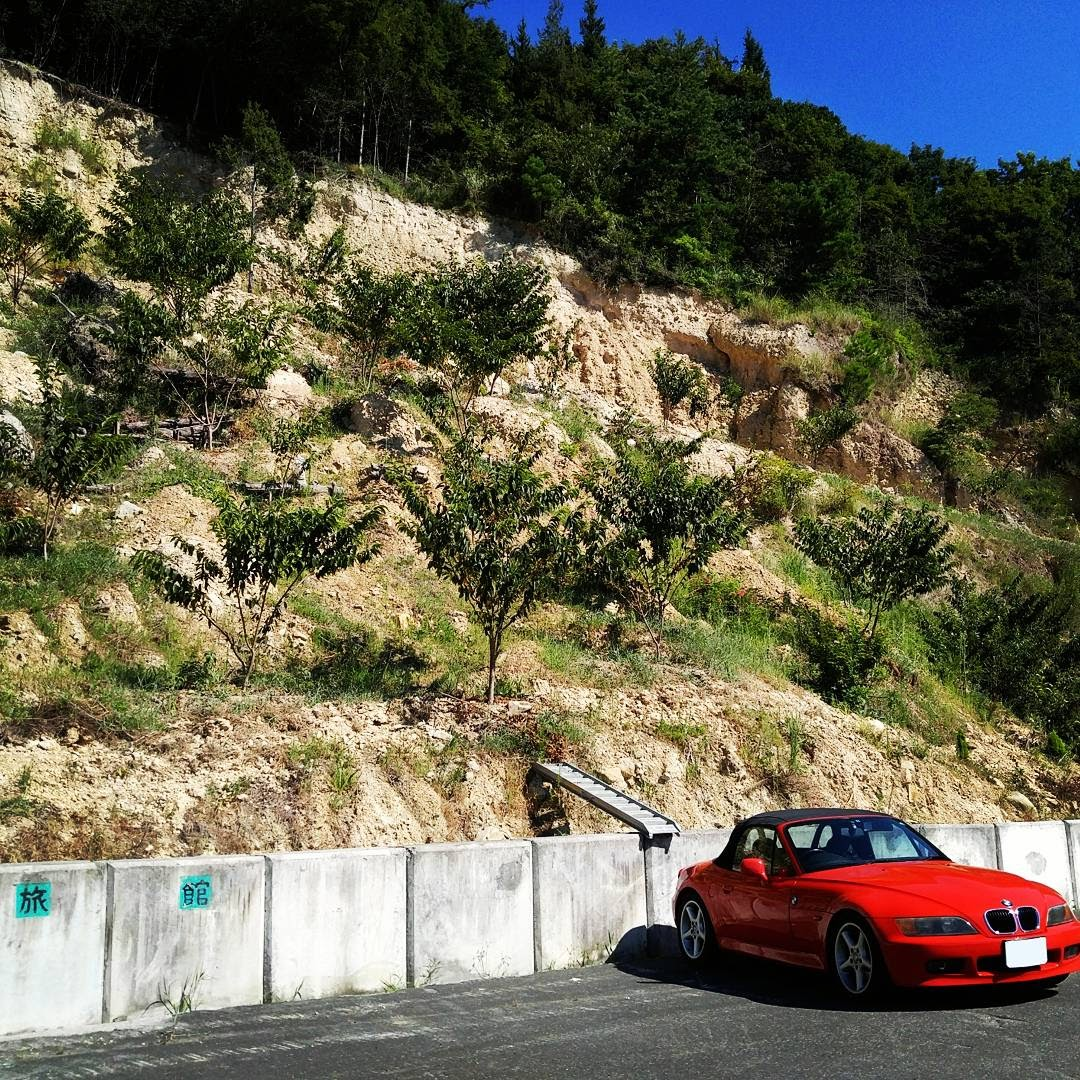
\includegraphics[width=5cm]{fig/sample.jpg}
                \caption{サンプル}
                \label{fig:sample}
            \end{figure}

        % 参考文献
        \begin{thebibliography}{1}
            \bibitem{sankou01} 「書籍」 著者 著 (2003年10月, XXXXX 発行)
        \end{thebibliography}
\end{document}
